\documentclass[11pt,preprint, authoryear]{elsarticle}

\usepackage{lmodern}
%%%% My spacing
\usepackage{setspace}
\setstretch{1.2}
\DeclareMathSizes{12}{14}{10}{10}

% Wrap around which gives all figures included the [H] command, or places it "here". This can be tedious to code in Rmarkdown.
\usepackage{float}
\let\origfigure\figure
\let\endorigfigure\endfigure
\renewenvironment{figure}[1][2] {
    \expandafter\origfigure\expandafter[H]
} {
    \endorigfigure
}

\let\origtable\table
\let\endorigtable\endtable
\renewenvironment{table}[1][2] {
    \expandafter\origtable\expandafter[H]
} {
    \endorigtable
}


\usepackage{ifxetex,ifluatex}
\usepackage{fixltx2e} % provides \textsubscript
\ifnum 0\ifxetex 1\fi\ifluatex 1\fi=0 % if pdftex
  \usepackage[T1]{fontenc}
  \usepackage[utf8]{inputenc}
\else % if luatex or xelatex
  \ifxetex
    \usepackage{mathspec}
    \usepackage{xltxtra,xunicode}
  \else
    \usepackage{fontspec}
  \fi
  \defaultfontfeatures{Mapping=tex-text,Scale=MatchLowercase}
  \newcommand{\euro}{€}
\fi

\usepackage{amssymb, amsmath, amsthm, amsfonts}

\def\bibsection{\section*{References}} %%% Make "References" appear before bibliography


\usepackage[round]{natbib}

\usepackage{longtable}
\usepackage[margin=2.3cm,bottom=2cm,top=2.5cm, includefoot]{geometry}
\usepackage{fancyhdr}
\usepackage[bottom, hang, flushmargin]{footmisc}
\usepackage{graphicx}
\numberwithin{equation}{section}
\numberwithin{figure}{section}
\numberwithin{table}{section}
\setlength{\parindent}{0cm}
\setlength{\parskip}{1.3ex plus 0.5ex minus 0.3ex}
\usepackage{textcomp}
\renewcommand{\headrulewidth}{0.2pt}
\renewcommand{\footrulewidth}{0.3pt}

\usepackage{array}
\newcolumntype{x}[1]{>{\centering\arraybackslash\hspace{0pt}}p{#1}}

%%%%  Remove the "preprint submitted to" part. Don't worry about this either, it just looks better without it:
\makeatletter
\def\ps@pprintTitle{%
  \let\@oddhead\@empty
  \let\@evenhead\@empty
  \let\@oddfoot\@empty
  \let\@evenfoot\@oddfoot
}
\makeatother

 \def\tightlist{} % This allows for subbullets!

\usepackage{hyperref}
\hypersetup{breaklinks=true,
            bookmarks=true,
            colorlinks=true,
            citecolor=blue,
            urlcolor=blue,
            linkcolor=blue,
            pdfborder={0 0 0}}


% The following packages allow huxtable to work:
\usepackage{siunitx}
\usepackage{multirow}
\usepackage{hhline}
\usepackage{calc}
\usepackage{tabularx}
\usepackage{booktabs}
\usepackage{caption}


\newenvironment{columns}[1][]{}{}

\newenvironment{column}[1]{\begin{minipage}{#1}\ignorespaces}{%
\end{minipage}
\ifhmode\unskip\fi
\aftergroup\useignorespacesandallpars}

\def\useignorespacesandallpars#1\ignorespaces\fi{%
#1\fi\ignorespacesandallpars}

\makeatletter
\def\ignorespacesandallpars{%
  \@ifnextchar\par
    {\expandafter\ignorespacesandallpars\@gobble}%
    {}%
}
\makeatother

\newenvironment{CSLReferences}[2]{%
}

\urlstyle{same}  % don't use monospace font for urls
\setlength{\parindent}{0pt}
\setlength{\parskip}{6pt plus 2pt minus 1pt}
\setlength{\emergencystretch}{3em}  % prevent overfull lines
\setcounter{secnumdepth}{5}

%%% Use protect on footnotes to avoid problems with footnotes in titles
\let\rmarkdownfootnote\footnote%
\def\footnote{\protect\rmarkdownfootnote}
\IfFileExists{upquote.sty}{\usepackage{upquote}}{}

%%% Include extra packages specified by user

%%% Hard setting column skips for reports - this ensures greater consistency and control over the length settings in the document.
%% page layout
%% paragraphs
\setlength{\baselineskip}{12pt plus 0pt minus 0pt}
\setlength{\parskip}{12pt plus 0pt minus 0pt}
\setlength{\parindent}{0pt plus 0pt minus 0pt}
%% floats
\setlength{\floatsep}{12pt plus 0 pt minus 0pt}
\setlength{\textfloatsep}{20pt plus 0pt minus 0pt}
\setlength{\intextsep}{14pt plus 0pt minus 0pt}
\setlength{\dbltextfloatsep}{20pt plus 0pt minus 0pt}
\setlength{\dblfloatsep}{14pt plus 0pt minus 0pt}
%% maths
\setlength{\abovedisplayskip}{12pt plus 0pt minus 0pt}
\setlength{\belowdisplayskip}{12pt plus 0pt minus 0pt}
%% lists
\setlength{\topsep}{10pt plus 0pt minus 0pt}
\setlength{\partopsep}{3pt plus 0pt minus 0pt}
\setlength{\itemsep}{5pt plus 0pt minus 0pt}
\setlength{\labelsep}{8mm plus 0mm minus 0mm}
\setlength{\parsep}{\the\parskip}
\setlength{\listparindent}{\the\parindent}
%% verbatim
\setlength{\fboxsep}{5pt plus 0pt minus 0pt}



\begin{document}



\begin{frontmatter}  %

\title{Analysing Taylor Swift's Music: Exploring Album Popularity, Song
Characteristics, and Predicting Top Hits}

% Set to FALSE if wanting to remove title (for submission)




\author[Add1]{Gabriella Neilon}
\ead{22581340@sun.ac.za}





\address[Add1]{Stellenbosch University}

\cortext[cor]{Corresponding author: Gabriella Neilon}


\vspace{1cm}


\begin{keyword}
\footnotesize{
Taylor Swift \sep Random Forest Algorithm \sep Song Prediction \\
\vspace{0.3cm}
}
\end{keyword}



\vspace{0.5cm}

\end{frontmatter}

\setcounter{footnote}{0}



%________________________
% Header and Footers
%%%%%%%%%%%%%%%%%%%%%%%%%%%%%%%%%
\pagestyle{fancy}
\chead{}
\rhead{}
\lfoot{}
\rfoot{\footnotesize Page \thepage}
\lhead{}
%\rfoot{\footnotesize Page \thepage } % "e.g. Page 2"
\cfoot{}

%\setlength\headheight{30pt}
%%%%%%%%%%%%%%%%%%%%%%%%%%%%%%%%%
%________________________

\headsep 35pt % So that header does not go over title




\hypertarget{background}{%
\section{\texorpdfstring{Background
\label{Background}}{Background }}\label{background}}

This report focuses on Taylor Swift, one of the most influential and
acclaimed artists of our time. With a remarkable career spanning across
country and pop genres, Taylor Swift has left an indelible mark on the
music industry, garnering 12 Grammy Awards and a massive fan base.The
main objective of this analysis is to predict the top 5 singles from her
latest album, \emph{Midnights (3am Edition)}, which was released in
October 2022. By analysing a combination of factors, including the
album's overall popularity and the distinctive characteristics of each
song, I aim to identify the tracks that have the potential make a
significant impact on the charts. By delving into Taylor Swift's musical
journey and employing predictive modeling techniques, this analysis
offers insights and predictions regarding the potential success of her
latest album's singles.

\hypertarget{data-methodology}{%
\section{\texorpdfstring{Data \& Methodology
\label{Data & Methodology}}{Data \& Methodology }}\label{data-methodology}}

\hypertarget{data}{%
\subsection*{Data}\label{data}}
\addcontentsline{toc}{subsection}{Data}

The dataset used in this analysis is the ``Taylor Swift Spotify''
dataset obtained from \emph{Kaggle}. It includes various attributes for
each song, such as the release date, song length, popularity
(represented as a percentage based on Spotify's algorithm), danceability
(a measure of how suitable a track is for dancing), acousticness, energy
(a measure of intensity and activity), instrumentalness (indicating the
presence of vocals in the song), liveness (the probability of the song
being recorded with a live audience), loudness (the volume level of the
music), speechiness (presence of spoken words in the track), valence (a
measure of the song's emotional tone), and tempo (beats per minute).

To simplify the analysis, only the deluxe editions and ``Taylor's
Version'' albums are selected. ``Taylor's Version'' refers to the music
that Taylor Swift owns and has re-recorded. This selection helps to
minimise potential bias in the data, considering that Taylor Swift's
popularity has likely increased over time, and these albums contain more
songs. By including these versions, the analysis levels the playing
field among all the albums. Additionally, a target variable called
``hit'' was engineered using binary encoding. A song is coded as 1 if it
was classified as a hit in the respective albums, based on the
popularity scores, and 0 if not.

\hypertarget{methodology}{%
\subsection*{Methodology}\label{methodology}}
\addcontentsline{toc}{subsection}{Methodology}

In order to predict her next top hits on her newest album, I employed
the \emph{random forest algorithm}. The \emph{random forest algorithm}
was chosen to make the ``next hit prediction'' as it provides accurate
predictions and efficiently handles large datasets.The strength of this
model lies in its ``social cognition'' of individual decision trees that
work together. Each decision tree is created by looking at different
features or characteristics of the data and finding the best split at
each step. When you want to make a prediction using the Random Forest,
you ask all the decision trees for their opinions, and then take a
majority vote. Each tree gets one vote, and the majority prediction
becomes the final prediction of the Random Forest. This way, the Random
Forest combines the strengths and insights of multiple decision trees to
make a more accurate prediction.Even if some trees are wrong, the
majority of the correct trees guide the collection to the right
direction

The \emph{random forest algorithm} consists of an ensemble of decision
trees. The ensemble, called a `forest,' is trained using bagging or
bootstrap aggregating. Bagging is a technique that improves the accuracy
of machine learning algorithms by combining their predictions. The
algorithm makes predictions by averaging or taking the mean of the
outputs from multiple decision trees. Increasing the number of trees
enhances the precision of the predictions. Random forest overcomes the
limitations of a single decision tree algorithm. It mitigates
overfitting issues and improves accuracy. Decision trees are built based
on entropy and information gain. Entropy measures uncertainty, while
information gain quantifies the reduction in uncertainty of the target
variable given independent variables. A higher information gain
indicates a greater reduction in uncertainty (entropy). Entropy and
information gain are crucial for splitting branches, a vital step in
building decision trees. The key characteristic of the \emph{random
forest algorithm} lies in the random selection of root and splitting
nodes. The random forest utilises ``bagging'' to generate predictions.
Bagging involves using different samples of training data rather than a
single sample. Each decision tree produces different outputs based on
the training data fed into the \emph{random forest algorithm}. These
outputs are ranked, and the highest-ranked output becomes the final
prediction.

\hypertarget{descriptive-statistics}{%
\subsection*{Descriptive Statistics}\label{descriptive-statistics}}
\addcontentsline{toc}{subsection}{Descriptive Statistics}

In Figure \ref{Figure1}, I present a comprehensive visual representation
of Taylor Swift's discography, showcasing the popularity of each album
and the emotions evoked by their most popular songs. To capture the
emotional essence, I conducted feature engineering by categorizing songs
as either ``Happy'' or ``Sad'' based on their valence score. Songs with
a valence score below 0.5 are classified as ``Sad,'' while those equal
to or above 0.5 are deemed ``Happy.''

\begin{figure}[H]

{\centering 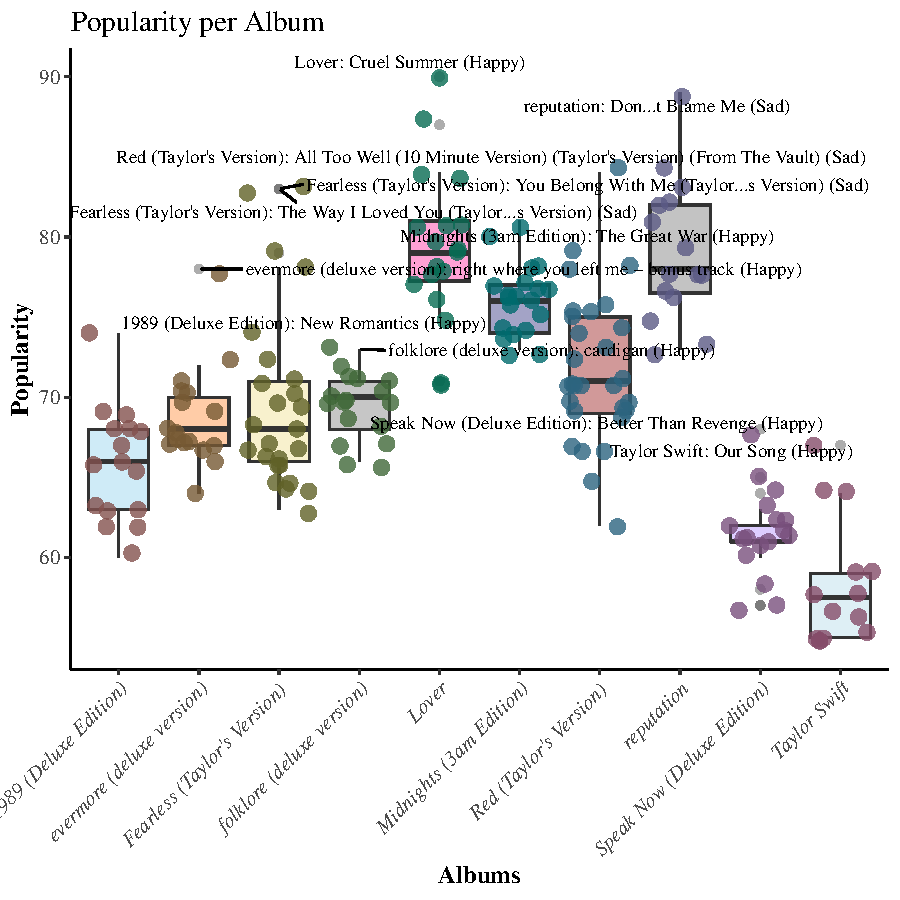
\includegraphics{Taylor-Swift-Report_files/figure-latex/Figure1-1} 

}

\caption{Popularity per Album \label{Figure1}}\label{fig:Figure1}
\end{figure}

The results reveal that Taylor Swift's most popular album, as indicated
by its overall popularity and the emotions it elicits, is
``reputation''. This is followed closely by the album ``Lover'' and her
latest release, ``Midnights (3am Edition)''. On the other hand, her
earlier albums, such as ``Taylor Swift'' and ``Speak Now,'' exhibit
comparatively lower popularity. This observation suggests that
popularity is influenced by the release date, with Taylor Swift's later
albums enjoying greater recognition, possibly reflecting her ascent to
fame over the years.

The subsequent visual representation (Figure \ref{Figure2}) explores the
shared characteristics found among the top 5 most popular songs from
each of Taylor Swift's albums. By identifying these common traits, I
further investigate the composition of the albums using these
influential characteristics. This analysis is presented in Figure
\ref{Figure3}.

\begin{figure}[H]

{\centering 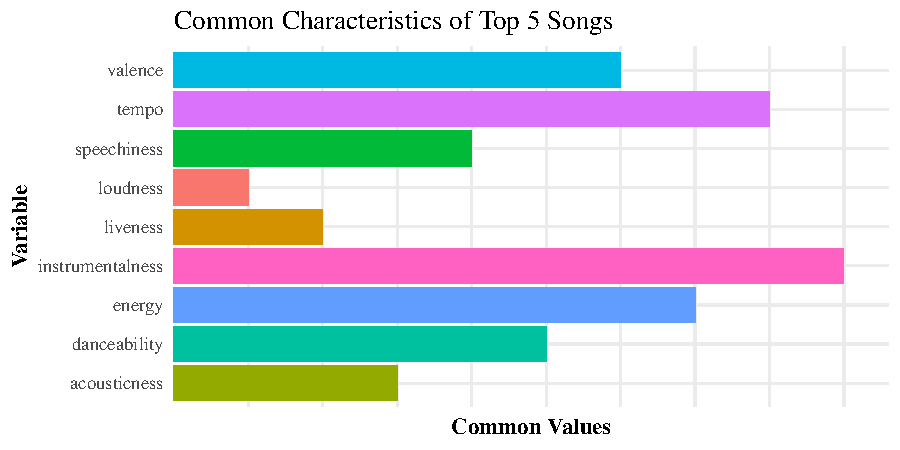
\includegraphics{Taylor-Swift-Report_files/figure-latex/Figure2-1} 

}

\caption{Common Characteristics of Top 5 Songs \label{Figure2}}\label{fig:Figure2}
\end{figure}

\begin{figure}[H]

{\centering 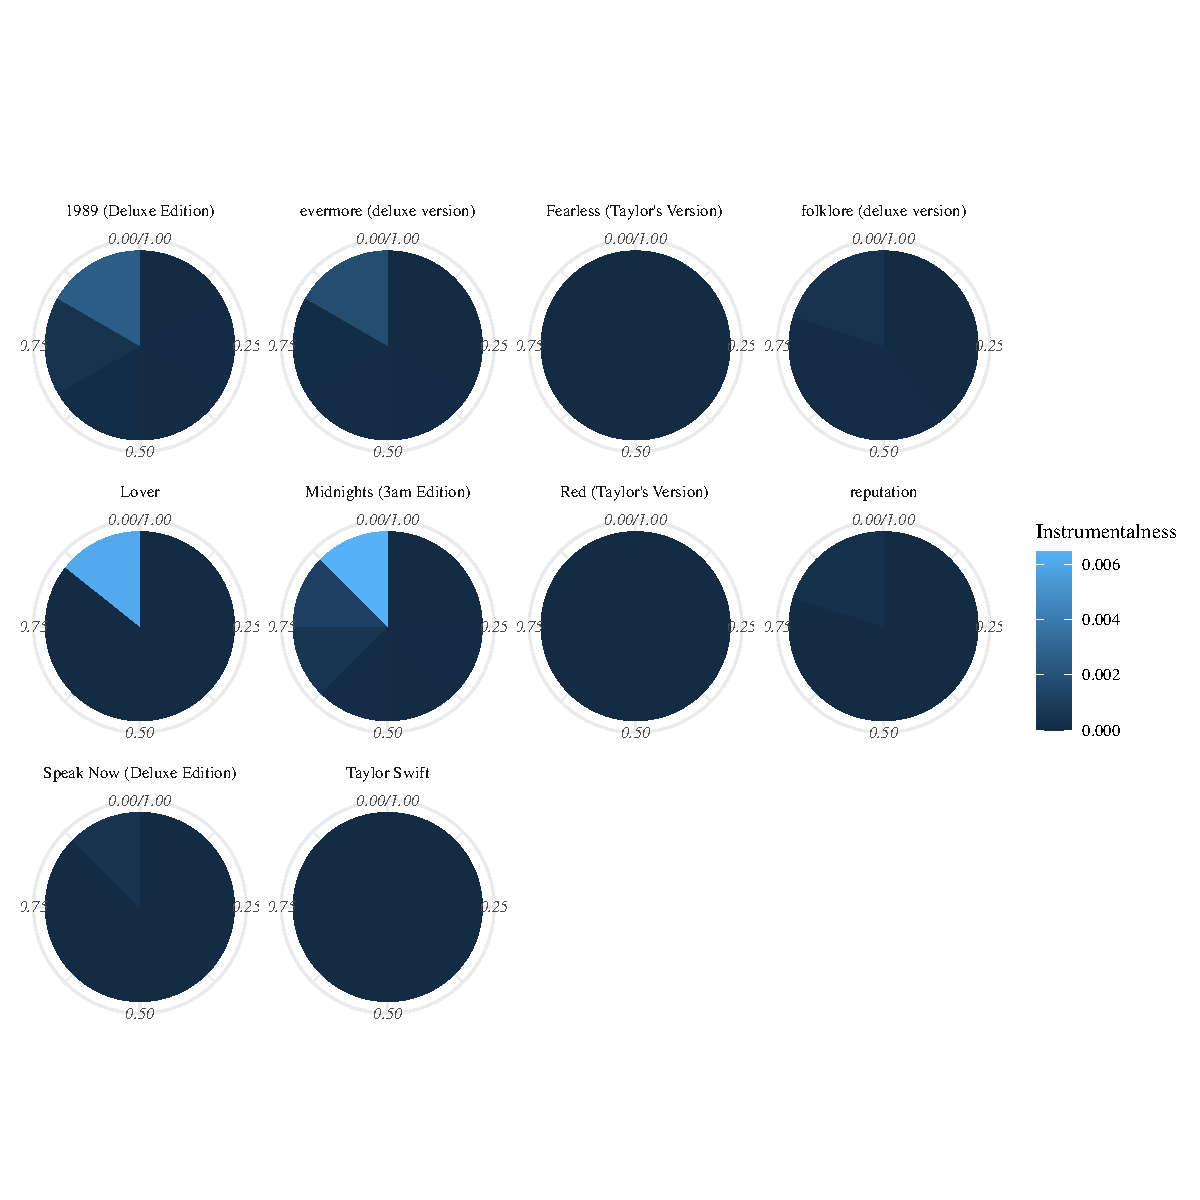
\includegraphics[angle=90]{Taylor-Swift-Report_files/figure-latex/Figure3-1} 

}

\caption{Common Characteristics of Top 5 Songs Concentration \label{Figure3}}\label{fig:Figure3-1}
\end{figure}
\begin{figure}[H]

{\centering 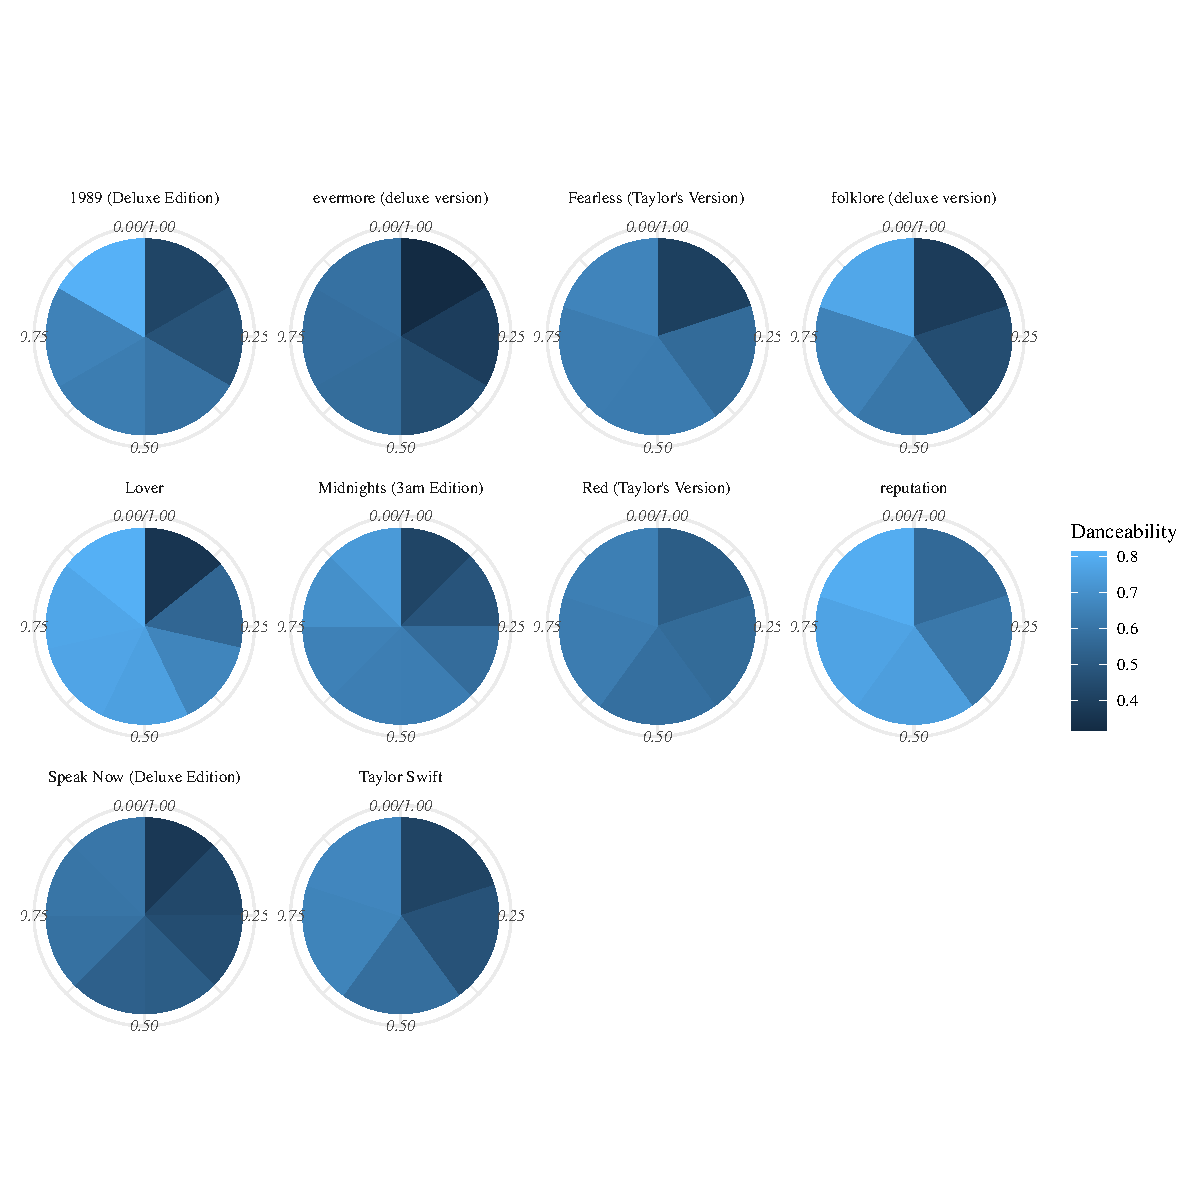
\includegraphics[angle=90]{Taylor-Swift-Report_files/figure-latex/Figure3-2} 

}

\caption{Common Characteristics of Top 5 Songs Concentration \label{Figure3}}\label{fig:Figure3-2}
\end{figure}
\begin{figure}[H]

{\centering 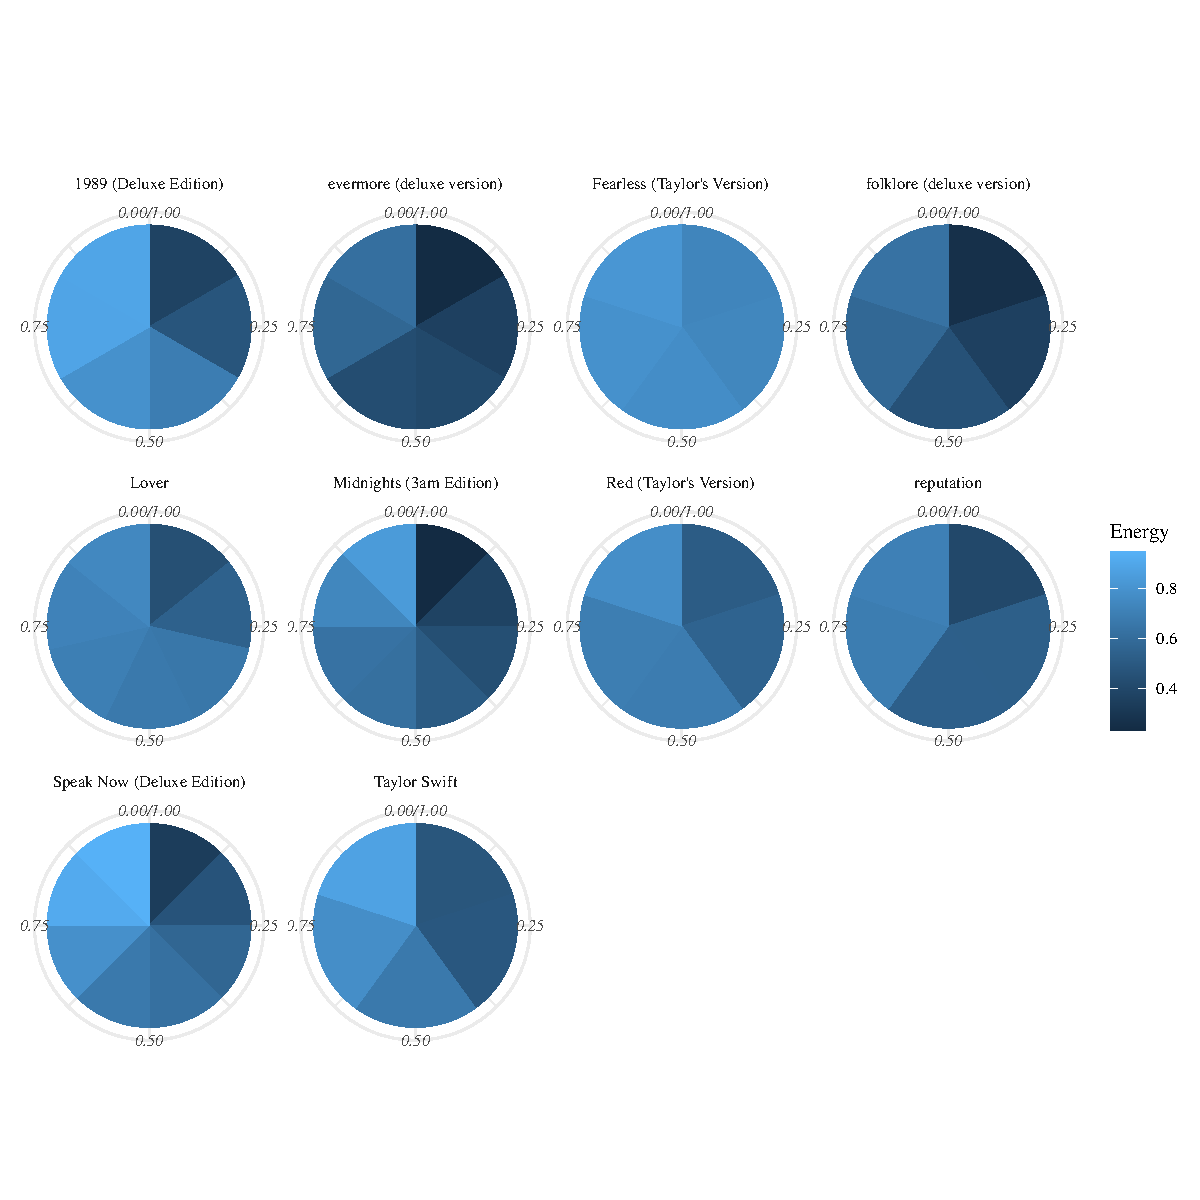
\includegraphics[angle=90]{Taylor-Swift-Report_files/figure-latex/Figure3-3} 

}

\caption{Common Characteristics of Top 5 Songs Concentration \label{Figure3}}\label{fig:Figure3-3}
\end{figure}

Generally, Taylor Swift's albums exhibit relatively low levels of
\emph{instrumentalness}, except for the albums ``Lover'' and ``Midnights
(3am Edition),'' which have already established themselves as among her
most popular works. This suggests that instrumental elements play a
significant role in the appeal and success of these particular albums.
In Figure \ref{Figure1}, it is observed that albums with lower overall
popularity tend to exhibit lower levels of \emph{energy}, while those
with higher popularity showcase higher levels of \emph{danceability}.
These findings highlight the connection between specific musical
attributes and the overall reception of Taylor Swift's albums.

\hypertarget{results}{%
\section{\texorpdfstring{Results
\label{Results}}{Results }}\label{results}}

\hypertarget{baseline-model}{%
\subsection*{Baseline Model}\label{baseline-model}}
\addcontentsline{toc}{subsection}{Baseline Model}

This model employs the default parameters, with the test data
representing Taylor Swift's latest album, ``Midnights (3am Edition),''
while the train data encompasses all of her previous works leading up to
the release of her newest album.

\begin{longtable}[]{@{}l@{}}
\caption{Baseline Model}\tabularnewline
\toprule()
Song Name \\
\midrule()
\endfirsthead
\toprule()
Song Name \\
\midrule()
\endhead
The Great War \\
Would've, Could've, Should've \\
Maroon \\
Snow On The Beach (feat. Lana Del Rey) \\
High Infidelity \\
\bottomrule()
\end{longtable}

Based on this model, the predicted top 5 singles (``hits'') for her next
releases are anticipated to be \emph{Maroon}, \emph{Snow On The Beach
(feat. Lana Del Rey)}, \emph{The Great War}, \emph{Would've, Could've,
Should've}, and \emph{Anti-Hero}.

\hypertarget{hypertuned-model}{%
\subsection*{Hypertuned Model}\label{hypertuned-model}}
\addcontentsline{toc}{subsection}{Hypertuned Model}

In this model, I aim to find the optimal configuration for predicting
the next top 5 ``hits'' by exploring different combinations of
hyperparameters based on the lowest Root Mean Square Error (RMSE). From
this, at each split, the model randomly selects 10 variables to
determine the best split. Secondly, I ensure that each terminal node in
the decision trees contains at least one observation. Furthermore, I use
sampling with replacement, allowing each bootstrap sample used for
training individual trees to contain duplicate observations.
Additionally, I train each tree on a randomly sampled subset of the
training data, comprising 50\% of the observations. This random sampling
process contributes to the creation of diverse trees and helps reduce
correlation among them. Finally, I set a random seed of 123 to ensure
the reproducibility of the results. This ensures that when the model is
re-run, the same random seed is used, resulting in consistent outcomes.
After tuning the hyperparameters, the resulting ``best model'' achieves
a prediction error of 0.171, as indicated by the RMSE. This performance
metric assesses how accurately the model predicts the next top 5 hits
based on the chosen configuration of parameters.

\begin{longtable}[]{@{}l@{}}
\caption{Hypertuned Model}\tabularnewline
\toprule()
Song Name \\
\midrule()
\endfirsthead
\toprule()
Song Name \\
\midrule()
\endhead
Snow On The Beach (feat. Lana Del Rey) \\
Maroon \\
Would've, Could've, Should've \\
The Great War \\
Anti-Hero \\
\bottomrule()
\end{longtable}

After fine-tuning the hyperparameters, the resulting ``best model''
achieves a prediction error of 0.171, as indicated by the RMSE. The RMSE
serves as a performance metric, assessing the accuracy of the model in
predicting the next top 5 hits based on the selected parameter
configuration. Based on this model, the predicted top 5 singles
(``hits'') for her next releases are anticipated to be \emph{Snow On The
Beach (feat. Lana Del Rey)}, \emph{Maroon}, \emph{Would've, Could've,
Should've}, \emph{The Great War}, and \emph{Anti-Hero}.

\hypertarget{feature-interpretation}{%
\subsection*{Feature Interpretation}\label{feature-interpretation}}
\addcontentsline{toc}{subsection}{Feature Interpretation}

In my analysis, I explore two methods to assess the importance of
variables: \emph{impurity-based and permutation-based variable
importance}.The \emph{impurity-based approach} measures the importance
of a feature by evaluating how much the randomness in predictions is
reduced when splitting on that feature. It uses the impurity measure,
such as entropy, to quantify the disorder or lack of purity in a set of
samples. The underlying assumption is that an important feature will
lead to more effective splits, reducing impurity and improving
prediction accuracy.

On the other hand, \emph{permutation-based importance} also estimates
feature importance by evaluating the decrease in model performance when
the values of a feature are randomly permuted. This approach provides a
direct measure of a feature's contribution to the predictive power of
the model. It takes into account the impact of the feature within the
entire model, providing valuable insights.

\begin{figure}[H]

{\centering 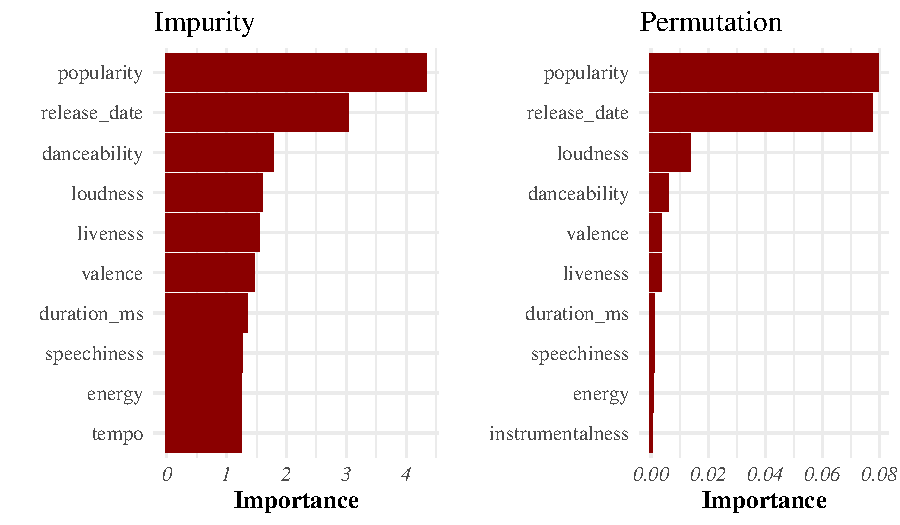
\includegraphics{Taylor-Swift-Report_files/figure-latex/Figure4-1} 

}

\caption{Impurity-based and Permutation-based Performance \label{Figure4}}\label{fig:Figure4}
\end{figure}

From both the \emph{impurity-based and permutation-based importance}
analyses, certain characteristics stand out as significant. These
include \emph{popularity, release date, loudness, and danceability}.
These findings align with my previous hypothesis that Taylor Swift's
next album's hits will be influenced by her growth in fame over the
years. Since ``hit'' classification is based on popularity, it makes
sense that the next hits will be closely linked to the songs'
popularity. Additionally, consistent with the descriptive statistics
from Figure \ref{Figure3}, danceability emerges as a key feature in her
most popular albums.

\hypertarget{model-performance}{%
\subsection*{Model Performance}\label{model-performance}}
\addcontentsline{toc}{subsection}{Model Performance}

The area under the ROC curve (AUC) is a widely used metric for assessing
the overall performance of the model. It quantifies the model's ability
to assign higher scores to positive instances than negative instances.
An AUC value of 0.5 suggests a random classifier, meaning the model
performs no better than random guessing. Conversely, an AUC value of 1
indicates a perfect classifier, where the model perfectly distinguishes
between positive and negative instances.

\begin{figure}[H]

{\centering 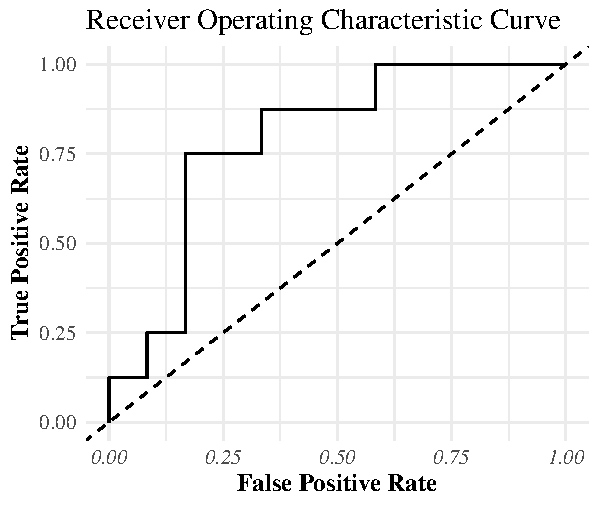
\includegraphics{Taylor-Swift-Report_files/figure-latex/Figure5-1} 

}

\caption{Receiver Operating Characteristic Curve \label{Figure5}}\label{fig:Figure5}
\end{figure}

The hypertuned \emph{best model} achieved an AUC value of 0.7917, which
indicates that its performance surpasses that of a random classifier.
This means that the model is highly proficient in making accurate
predictions and effectively distinguishing between positive and negative
instances in the classification task at hand. The high AUC score
demonstrates the model's strong discriminatory power and its ability to
provide reliable classifications. Consequently, we can conclude that the
model is an effective classifier.

\hypertarget{conclusion}{%
\section{Conclusion}\label{conclusion}}

Based on the analysis performed, it can be concluded that the model has
shown success in predicting the next top 5 singles from Taylor Swift's
discography. The evaluation of the model's performance using the ROC
curve revealed that it outperforms a random classifier, indicating its
capability to make accurate predictions and serve as a reliable
classifier. Although there is a slight difference in the ordering of the
songs between the baseline model and the hypertuned model, both models
predict the same top 5 songs. It is noteworthy that the song
``Anti-Hero'' was indeed Taylor Swift's first single from her newest
album, which highlights the model's ability to capture upcoming hits.
Furthermore, while the remaining songs predicted by the model have not
been officially announced as singles, their inclusion in the top 5
aligns with the preferences of the devoted Taylor Swift fan community,
known as ``Swiftie''. As a dedicated ``Swiftie'' myself, I can affirm
that these songs hold high favourability among ``Swiftie'' enthusiasts
based on their online discussions and interactions.

\newpage

\bibliography{Tex/ref}





\end{document}
